\documentclass[./main.tex]{subfiles}

\begin{document}

虽然 Haskell 的纯性带来了非常多的便利,但是在处理某些问题时,我们需要不同与命令式语言那样的方式来解决。由于引用透明,Haskell 中相同的值时没有区别的。

如果我们有一颗树的节点都是五,当我们想要将它们其中一个变为六时,我们必须要知道到底究竟是哪个五想要变成六。也就是说必须知道其位置。在不纯的语言中,仅需
知道其内存地址,并改变它。然而在 Haskell 中,一个五跟其它的五并无差异,因此我们不能通过内存地址来进行辨别。同样的,我们也不能真的\textit{修改}任何
东西;当我们说改变一颗树,真正的意思其实是接受一棵树,返回一个与原始树相近的树,且只有细微的不同。

一种方法就是从树的根部记住通向节点的路径,但是这样效率低下。如果想要修改一个临近之前修改过的节点,我们又要从头来过!

本章我们将学习如何集中注意在某个数据结构上,使得改变数据结构与遍历的动作变得高效。

\subsection*{走二元树}

首先是之前章节介绍过的树的定义:

\begin{lstlisting}[language=Haskell]
  data Tree a = Empty | Node a (Tree a) (Tree a) deriving (Show)
\end{lstlisting}

下面是一个数的例子:

\begin{lstlisting}[language=Haskell]
  freeTree :: Tree Char
  freeTree =
    Node
      'P'
      ( Node
          'O'
          (Node 'L' (Node 'N' Empty Empty) (Node 'T' Empty Empty))
          (Node 'Y' (Node 'S' Empty Empty) (Node 'A' Empty Empty))
      )
      ( Node
          'L'
          (Node 'W' (Node 'C' Empty Empty) (Node 'R' Empty Empty))
          (Node 'A' (Node 'A' Empty Empty) (Node 'C' Empty Empty))
      )
\end{lstlisting}

\newpage
其图形如下:

\begin{figure}[h]
  \centering
  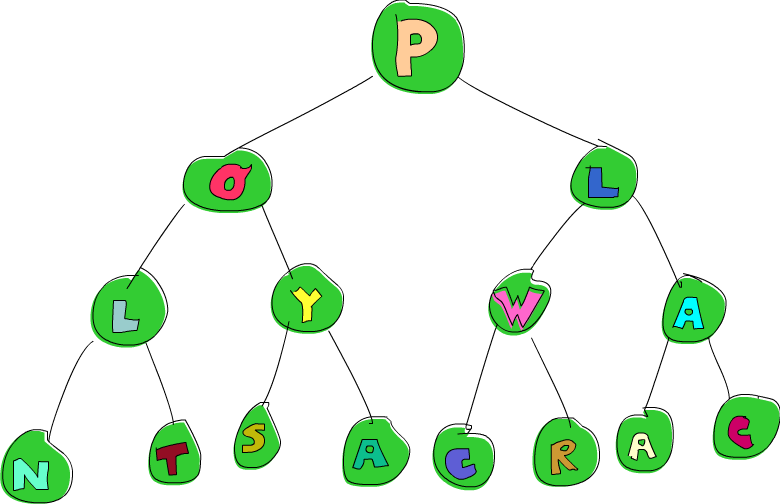
\includegraphics[width=0.8\textwidth]{\subfix{./images/pollywantsa.png}}
\end{figure}

注意到\acode{W}在树中的位置了吗?我们想要将其变为\acode{P}。那么该怎么做呢?其中一种方式就是通过对树进行模式匹配,直到第一次找到该元素的位置,然后再
进行修改:

\begin{lstlisting}[language=Haskell]
  changeTop :: Tree Char -> Tree Char
  changeTop (Node x l (Node y (Node _ m n) r)) = Node x l (Node y (Node 'P' m n) r)
\end{lstlisting}

呃这不仅丑陋而且还令人迷惑。那么发生了什么?首先是模式匹配根元素\acode{x}(即\acode{'P'})以及左子树\acode{l},而对于右子树再次进行模式匹配,以此类推,
最终替换\acode{'W'}成为\acode{'P'}。

那么有没有更好的办法呢?不如构建一个函数,接受一棵树以及一个方向列表。方向即\acode{L}或\acode{R}:

\begin{lstlisting}[language=Haskell]
  data Direction = L | R deriving (Show)

  type Directions = [Direction]

  changeToP :: Directions -> Tree Char -> Tree Char
  changeToP (L : ds) (Node x l r) = Node x (changeToP ds l) r
  changeToP (R : ds) (Node x l r) = Node x l (changeToP ds r)
  changeToP [] (Node _ l r) = Node 'P' l r
\end{lstlisting}

如果方向列表的第一个元素是\acode{L},我们将构建一颗与旧树一样的树,只不过左子树会有元素变为\acode{'P'}。当递归调用\acode{changeToP},则传入列表尾部,
因为头部已经被消费了。\acode{R}同理。如果列表为空,意味着到达了目的地,返回一个新的树,其根被改为\acode{'P'}。

为了避免打印出整棵树,让我们构建一个函数,接受一个方向的列表,返回目的地的元素:

\begin{lstlisting}[language=Haskell]
  elemAt :: Directions -> Tree a -> a
  elemAt (L : ds) (Node _ l _) = elemAt ds l
  elemAt (R : ds) (Node _ _ r) = elemAt ds r
  elemAt [] (Node x _ _) = x
\end{lstlisting}

这个函数跟\acode{changeToP}很像,只不过不是记住路径并重构树,而是忽略所有经过只记住目的地。这里修改了\acode{'W'}至\acode{'P'},检查是否修改成功:

\begin{lstlisting}[language=Haskell]
  ghci> let newTree = changeToP [R,L] freeTree
  ghci> elemAt [R,L] newTree
  'P'
\end{lstlisting}

虽然这个技巧可能看起来很酷,但是它还是低效,特别是当我们需要频繁的修改元素时。假设我们有一个很大的树,一个指向了树底部元素的很长的方向列表。那么当我们修改
一个元素后,又要修改另一个临近的元素,我们又得重头开始一直走到树的底部!

\subsection*{留下面包屑的路径}

那么专注在一个子树,我们希望一个比方向列表更好的东西,避免总是从树的根部开始。那么如果从树根部开始,每次移动一步并留下印记,类似于留下面包屑会有帮助吗?
换言之,向左时记住向左,向右时记住向右。

为了表示面包屑,可以使用一个\acode{Direction}列表,由于我们留下的方向现在是相反的,为了区分\acode{Directions},我们称其为\acode{Breadcrumbs},

\begin{lstlisting}[language=Haskell]
  type Breadcrumbs = [Direction]
\end{lstlisting}

下面是一个接受一棵树以及面包屑的函数,当移动至左子树时,添加\acode{L}在列表头部:

\begin{lstlisting}[language=Haskell]
  goLeft :: (Tree a, Breadcrumbs) -> (Tree a, Breadcrumbs)
  goLeft (Node _ l _, bs) = (l, L : bs)
\end{lstlisting}

忽略根以及右子树,返回左子树以及在旧的面包屑头部添加了\acode{L}的新面包屑。下面是往右的函数:

\begin{lstlisting}[language=Haskell]
  goRight :: (Tree a, Breadcrumbs) -> (Tree a, Breadcrumbs)
  goRight (Node _ _ r, bs) = (r, R : bs)
\end{lstlisting}

现在使用这些函数来接受我们的\acode{freeTree},先是向右再向左:

\begin{lstlisting}[language=Haskell]
  ghci> goLeft (goRight (freeTree, []))
  (Node 'W' (Node 'C' Empty Empty) (Node 'R' Empty Empty),[L,R])
\end{lstlisting}

现在有了一个以\acode{'W'}为根的树,\acode{'C'}为左子树的根而\acode{'R'}为右子树的根,面包屑则为\acode{[L, R]},因为我们是先右后左。

我们可以定义一个\acode{-:}函数来将代码变得更可读:

\begin{lstlisting}[language=Haskell]
  x -: f = f x
\end{lstlisting}

它可以将函数的应用变为先写值,然后是\acode{-:}接着函数。那么改写以后就成了:

\begin{lstlisting}[language=Haskell]
  ghci> (freeTree, []) -: goRight -: goLeft
  (Node 'W' (Node 'C' Empty Empty) (Node 'R' Empty Empty),[L,R])
\end{lstlisting}

\subsubsection*{从后至前}

那么如果想要反向走树呢?根据面包屑我们可以知道当前树是其父树的左子树,然后更上一层则是右子树。仅仅如此,它并没有告知当前子树其父足够的信息,让我们
能够继续往树上走。除了单纯记录方向之外,还必须把其它的数据记录下来。这个案例中就是子树的父信息以及其右子树。

一般而言,一个面包屑有足够的信息用于重建父节点。所以它应该包含所有没有选择的路径信息,记录我们走过的方向;同时它不应该包含现在关注的子树,因为它已经在
元组的第一部分了,如果也记录下来就会有重复的信息。

现在来修改一下面包屑的定义,让它包含我们之前丢掉的信息:

\begin{lstlisting}[language=Haskell]
  data Crumb a = LeftCrumb a (Tree a) | RightCrumb a (Tree a) deriving (Show)
\end{lstlisting}

用\acode{LeftCrumb}来包含我们走过的右子树,以及没走过的右子树,而不是仅仅写个\acode{L},\acode{RightCrumb}同理。

这些面包屑现在包含了重构树所需的所有信息。它们像是软盘一样存储了走过的路径,而不仅仅只有方向。

基本而言可以将每个面包屑视为一个树的节点,树的节点有一个洞,当向树的更深处走,面包屑携带所有走过的信息,除了当前关注的子树被记录在洞那里。

我们也要把\acode{Breadcrumbs}的类型别名改成:

\begin{lstlisting}[language=Haskell]
  type Breadcrumbs' a = [Crumb a]
\end{lstlisting}

接着修改\acode{goLeft}以及\acode{goRight}来记录没有走过的路径信息,而不是像之前那样忽略掉:

\begin{lstlisting}[language=Haskell]
  goLeft' :: (Tree a, Breadcrumbs' a) -> (Tree a, Breadcrumbs' a)
  goLeft' (Node x l r, bs) = (l, LeftCrumb x r : bs)
\end{lstlisting}

类似于之前的\acode{goLeft},不同于仅仅添加一个\acode{L}在面包屑列表头部,而是添加了一个\acode{LeftCrumb}记录从左走过,以及未走过的右子树。

注意该函数假设了当前注意的树并不为\acode{Empty}。一颗空树是不会有任何子树的,所以如果在一颗空树上向左走,异常将会出现,因为对\acode{Node}的
匹配不成功,且没有额外去匹配\acode{Empty}。

\acode{goRight}也类似:

\begin{lstlisting}[language=Haskell]
  goRight' :: (Tree a, Breadcrumbs' a) -> (Tree a, Breadcrumbs' a)
  goRight' (Node x l r, bs) = (r, RightCrumb x l : bs)
\end{lstlisting}

现在有了向左和向右,我们就能具备了返回树根的能力了,以下是\acode{goUp}函数:

\begin{lstlisting}[language=Haskell]
  goUp :: (Tree a, Breadcrumbs' a) -> (Tree a, Breadcrumbs' a)
  goUp (t, LeftCrumb x r : bs) = (Node x t r, bs)
  goUp (t, RightCrumb x l : bs) = (Node x l t, bs)
\end{lstlisting}

该函数接受一个正在关注的树\acode{t},以及一个\acode{Breadcrumbs}用于检查最近的\acode{Crumb},如果是一个\acode{LeftCrumb},那么构建一颗新树,
而\acode{t}作为该树的左子树。这里通过两次模式匹配,首先是\acode{Breadcrumbs}的头,接着是\acode{LeftCrumb},拿到\acode{x}右子树\acode{r}
用来构建\acode{Node}剩余部分,并将剩下的\acode{Breadcrumbs}即\acode{bs}一并返回。

注意该函数在树的顶部会导致错误,稍后我们将用\acode{Maybe}单子来代表失败来进行改进。

有了一对元组\acode{Tree a}与\acode{Breadcrumbs a},我们便具备了所有重构的信息。这个模版可以让向上,向左以及向右变得简单很多。这样一对包含了关注的
部分以及其它信息的元组被称为 zipper。因此我们可以对其进行类型别名:

\begin{lstlisting}[language=Haskell]
  type Zipper a = (Tree a, Breadcrumbs' a)
\end{lstlisting}

\subsubsection*{操作当前注意的树}

现在我们有了向上与向下的移动,那么就可以构建一个函数用于修改 zipper 所关注的元素了:

\begin{lstlisting}[language=Haskell]
  modify :: (a -> a) -> Zipper a -> Zipper a
  modify f (Node x l r, bs) = (Node (f x) l r, bs)
  modify f (Empty, bs) = (Empty, bs)
\end{lstlisting}

如果关注在一个节点,通过函数\acode{f}修改其根元素;如果关注在一颗空树,则不做改动。测试:

\begin{lstlisting}[language=Haskell]
  ghci> let newFocus = modify (\_ -> 'P') (goRight (goLeft (freeTree,[])))
\end{lstlisting}

用可读性更好的\acode{-:}函数:

\begin{lstlisting}[language=Haskell]
  ghci> let newFocus = (freeTree,[]) -: goLeft -: goRight -: modify (\_ -> 'P')
\end{lstlisting}

接着是向上移动,替换字符为\acode{'X'}:

\begin{lstlisting}[language=Haskell]
  ghci> let newFocus2 = modify (\_ -> 'X') (goUp newFocus)
\end{lstlisting}

使用\acode{-:}:

\begin{lstlisting}[language=Haskell]
  ghci> let newFocus2 = newFocus -: goUp -: modify (\_ -> 'X')
\end{lstlisting}

向上移动很简单,因为面包屑的另一部分数据结构是没有关注的,不过它是倒转过来的,有点像是要把袜子反过来才能用那样。有了这些信息,我们便不用再从根走一遍,
而是从反过来的树顶部开始,将其部分翻转后再将其置为关注。

每个节点都有两个子树,即使这些子树是空树。所以当关注了一颗空的子树,可以将其替换为一颗非空子树,即叶节点:

\begin{lstlisting}[language=Haskell]
  attach :: Tree a -> Zipper a -> Zipper a
  attach t (_, bs) = (t, bs)
\end{lstlisting}

接受一颗树以及一个 zipper 并返回一个新的 zipper,其关注的被替换为接受的树。我们不仅能用这个方法来延展一棵树,还可以替换整个子树。通过\acode{attach}
来替换\acode{freeTree}最左的树:

\begin{lstlisting}[language=Haskell]
  ghci> let farLeft = (freeTree,[]) -: goLeft -: goLeft -: goLeft -: goLeft
  ghci> let newFocus = farLeft -: attach (Node 'Z' Empty Empty)
\end{lstlisting}

\subsubsection*{直接走到树顶端}

直接走到树顶端很简单:

\begin{lstlisting}[language=Haskell]
  topMost :: Zipper a -> Zipper a
  topMost (t,[]) = (t,[])
  topMost z = topMost (goUp z)
\end{lstlisting}

如果面包屑没了,那么就表示已经在树的根处了,并返回当前关注的树。

\subsection*{专注于列表}

% TODO

\begin{lstlisting}[language=Haskell]

\end{lstlisting}

\subsection*{一个简单的文件系统}

% TODO

\begin{lstlisting}[language=Haskell]

\end{lstlisting}

\subsection*{注意你的脚步}

% TODO

\begin{lstlisting}[language=Haskell]

\end{lstlisting}

\end{document}
